\documentclass[iop]{emulateapj}
\let\captionbox\relax
\usepackage{graphicx}
\bibliographystyle{apj}

%define general packages
\usepackage{epsfig}
\usepackage{rotating}
\usepackage{amsmath}
\usepackage{footnote}
\usepackage{courier}
\usepackage{color}
\usepackage{subfigure}



\begin{document}
\title{Ultraviolet to Infrared Star Formation Rate Indicators and Galaxy Environment}
\author{Nityasri Mandyam\altaffilmark{1} and Michael R. Blanton\altaffilmark{1}}
\altaffiltext{1}{Center for Cosmology and Particle Physics, Department of Physics, New York University, New York, NY $10003$}
\begin{abstract}
Star-forming galaxies preferentially populate isolated regions, while non-star-forming galaxies preferentially exist in groups and clusters. We investigate how this relationship depends on the star formation rate indicator using full UV to IR photometry for a local sample of galaxies (redshift $z \sim 0.05$) with ultraviolet and optical photometry from the NASA Sloan Atlas and infrared photometry from WISE. We measure the Specific Star Formation Rates (SSFR) in two independent ways: (a) using MAGPHYS, a complete UV to IR SED fitting method that models dust absorption and emission; (b) using purely the UV light to quantify star formation rates and accounting for dust attenuation from the ratio of fluxes in FUV and NUV bands. We estimate environments using projected aperture densities and distances to the $n^{th}$ nearest neighbor. We find that SSFR measured by including infrared emission is more closely related to the galaxy environments than the UV indicator.
\end{abstract}

\section{Introduction}


The formation history of galaxies is one of the most interesting puzzles in astronomy. The average star formation rates of galaxies have reduced with cosmic time (\citet{Mad98}, \underline{others? - Lilly et al?}) and star-forming galaxies ``transition" to red and quiescent ones\underline{(reference)}. Many mechanisms have been proposed to map out this process of galaxy evolution but there are many unsolved questions with regards to the nature and extent of the parameters that govern this. These mechanisms are known to be affected by the environment \underline{(Blanton, Moustakas)} and typically quiescent galaxies exist in dense regions today.\\

Study of this problem is limited by our poor understanding of star formation rate estimates. Although it is known that different spectral indicators contain signatures of star formation in them, often the spectrum of the galaxy is not readily available and we have to rely on converting photometric fluxes to meaningful star formation estimates. Fitting for the Spectral Energy Distribution (SED) of a galaxy using photometric data in various available bandpasses and applying the right bolometric corrections is one way of estimating the star formation rate and the star formation history of the galaxy. Another indicator of the amount of current star formation in a galaxy is its rest frame UV luminosity and converting the FUV-NUV fluxes into star formation rates is a popular method. However the presence of dust complicates matters as dust is known to absorb more in the UV/optical region of the galaxy spectrum and hence has a tendency to ``redden" the photometric data. The dust particles which are typically known to be polycyclic aromatic hydrocarbons and warm and cold grains reemit this light in the mid to far IR.\\

The effect of dust in diminishing UV luminosity has been studied and recent studies (\citet{Burg13}) have found that that in the nearby universe, almost $70\%$ of the FUV luminosity is obscured by dust on an average. And while mechanisms have been proposed to account for dust attenuation\underline{(Such as \citet{Sal07} and?)}, the reliance on UV SFR's extensively in the literature (\underline{cite Peng et al, Moustakas et al..?}) makes it important to understand how well the dust corrections for UV SFR estimates work, especially relative to other methods of estimating SFR.\\

Here, we examine a sample of galaxies whose UV-IR photometries are available and estimate the Star Formation rate in two independent ways. First we exploit the fact that we have UV to IR photometry and perform SED fitting using MAGPHYS \cite[]{daC08}, which accounts for dust by using a simple method of energy balance to obtain the Specific Star Formation Rates. The other method involves using purely UV photometry to estimate both star formation rate and dust attenuation by a prescription given by \citet{Sal07}. We also estimate the environments of our population and ask the following questions: Why and how do these different star formation estimators disagree with each other? Is there a particular region in the color-color phase space where either SFR indicator picks up the signal better? Which star formation rate estimator traces environment better? A reasonable assumption to make would be that the environment primarily correlates with the SFR itself rather than the relative impact of UV or IR emission. For this reason, studying this correlation will yield insights into the relative accuracy of each method.

\begin{figure*}
    \centering
	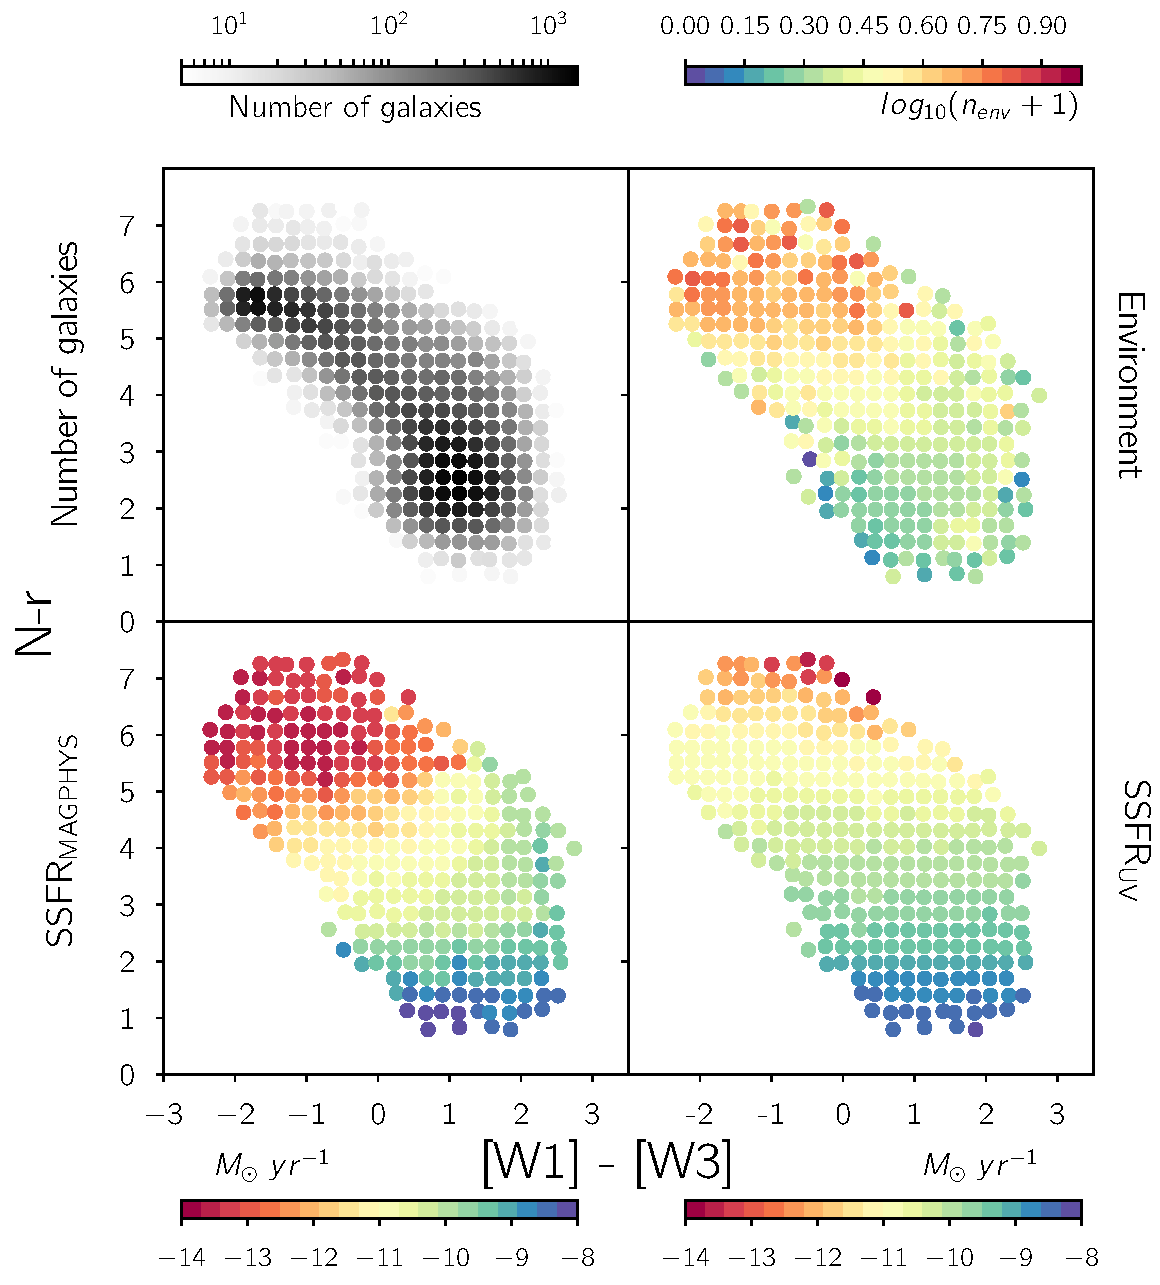
\includegraphics[width = 16 cm, height = 16 cm]{panel_plot.pdf}
	\caption{The SSFR measurements and environment shown in the color-color space: the measurements are represented by the colorbars and each point in the scatter plot is are the mean colors in each of the bins respectively; \emph{top left} shows the binning used to obtain the average fluxes - the gray scale displays the logarithmic number density in each of the bins; All bins with less than $5$ galaxies were discarded; \emph{top right} Environment:  In each bin the \textbf{volume density} is calculated from the average number of nearest neighbors in a projected cylinder ($r_{t} = 0.5 Mpc$ and $v_{los} = \pm 1000 km/s$); \emph{bottom left} the Specific Star Formation Rates obtained from MAGPHYS; \emph{bottom right} UV Specific Star Formation Rates estimated by using the method described in \citet{Sal07}.} 
\end{figure*}


\section{Data}

\subsection{Constructing a local sample spanning Ultraviolet to Infrared Imaging}


The sample on which we perform our measurements is based on the NSA catalog, a nearby galaxy sample which includes optical and ultraviolet imaging from SDSS and GALEX respectively. We use the currently public version of the NSA (http://nsatlas.org) whose redshift range extends up to $z = 0.055$ and includes SDSS(Data Release $6$) and GALEX imaging for galaxies. The total number of objects in the NSA catalogue is $\sim150,000$; however around $20\%$ of the objects do not have GALEX photometry.  \\


To obtain infrared imaging for the data we have photometrically matched the objects from the NSA with the WISE (Wide-Field Infrared Survey Explorer) data with k-corrected WISE magnitudes. Thus our sample in total contains $\sim75,000$ objects with absolute magnitudes in the UV ($F$ and $N$ bands), optical ($U$,$g$,$r$,$i$ and $z$ bands) and infrared ($W1$,$W2$, $W3$ and $W4$ bands). \\


\textbf{Add paragraph on Volume limited sample}\\
We imposed a volume limited cut on the absolute magnitude ( $-18.5 > M_{r}  > -24.5$) to get an environment determining population of $95638$ galaxies. After removing galaxies with zero/negative fluxes, we imposed a cut in optical ($7.5> N-r >=0 $) and infrared ($3.0> [W1]- [W3] >= -3.0$) colors to obtain $75476$ galaxies upon which the star formation rate measurements were then performed.\\



\section{Estimating the Specific Star Formation Rates}

\subsection{SED Fitting - MAGPHYS}

To understand the distribution of the Specific Star Formation Rates \textcolor{red}{(hereafter SSFR)} of our sample across the color-color space,  the photometric fluxes in bands  were normalized to an $r$-band flux of $1$ Jy. The galaxies were then binned along the $N-r$ - $[W1]-[W3]$ space ($25\times25$) and the mean flux in these bins were used for each band to obtain a ``template" for each bin in the color-color space.\\

MAGPHYS - Multi-wavelength Analysis of Galaxy Physical Properties \cite[]{daC08}  is a simple, largely empirical but physically motivated model to interpret the mid- and far-infrared spectral energy distributions of galaxies consistently with the emission at ultraviolet, optical and near-infrared wavelengths. For every input galaxy with a set of observed fluxes in different bands, MAGPHYS generates an optical and infrared library at that redshift and then samples all template spectra whose fluxes obey a simple principle of energy balance: that the amount of energy absorbed by dust in the UV/Optical matches \underline{within some tolerance?} the amount of infrared emission that is accounted for purely by dust. Once the templates have been subsampled thus, MAGPHYS uses chi-squared fitting to see which combination best reproduces the observed fluxes along with the likelihood for the distributions.\\

\begin{figure}
	\centering
		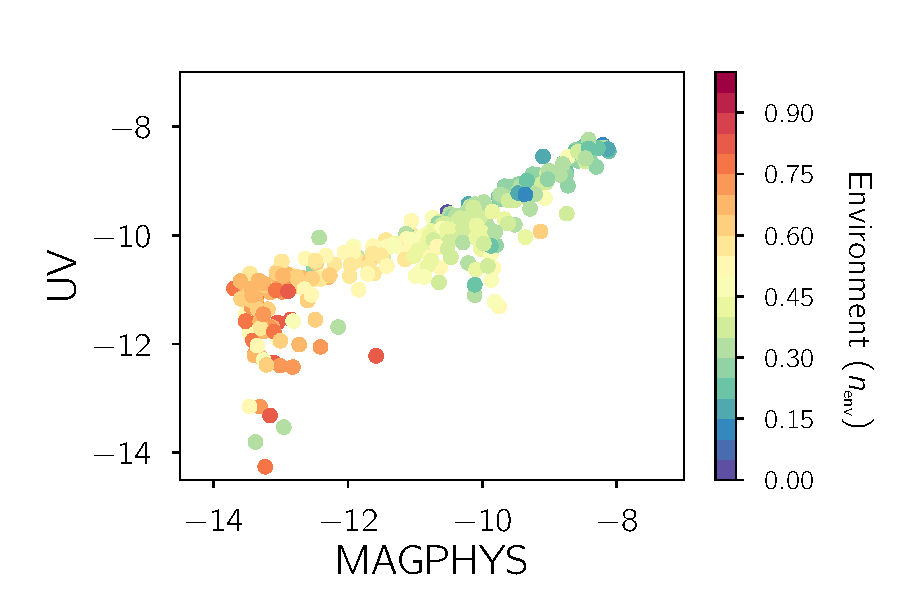
\includegraphics[width = 9 cm, height = 6.0 cm]{env_plot.pdf}
	\caption{The two star formation rate estimates (from Fig.$1$) plotted against each other as a function of the environment; We notice two distinct set of outliers that seem to have lower UV SSFR's but similar environments to the galaxy bins with the same MAGPHYS SSFR's.} 
\end{figure}

In order to circumvent the computational expense involved in fitting for every galaxy, we binned the galaxies along the color-color space and averaged the fluxes in each bin (which were normalized to an r band flux of $1 Jy$) thus generating a ``template galaxy" for each bin. The results for the specific star formation rates thus obtained are shown in Figure $2$ along with the number distribution of the galaxies across the chosen bins. Note that bins with $< 5$ galaxies were omitted as those regions of the color-color space are obviously under-sampled. \\




\subsection{UV Star Formation Rates}
The star formation rate of a galaxy is highly constrained by its UV luminosity. We use a simple method developed by \citet{Sal07} that exploits this feature and prescribes a star formation rate that is proportional to the UV luminosity (specifically the FUV band if we are looking at GALEX)  via the Kennicutt-Schmidt relation. Dust attenuation is also accounted for in this method by looking at the ratio of luminosities in the FUV and NUV bands.\\

\begin{figure*}
	\centering
		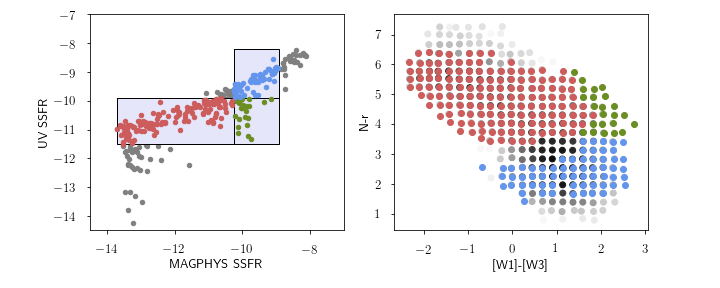
\includegraphics[width = 16 cm, height = 6.4 cm]{outliers.pdf}
	\caption{The outliers shown as a function of the Star Formation Rates as well as Optical and IR colors} 
\end{figure*}
According to the prescription \cite[]{Sal07}, the star formation rate can be given by:
$$ SFR = 1.08 \times 10^{-28}{L^{0}}_{FUV} $$
Where ${L^{0}}_{FUV}$ is the rest-frame FUV luminosity. This method accounts for dust attenuation of the FUV light as well by suggesting an attenuation factor $A_{\nu}$ which is obtained thus:

If $N-r \geq 4.0$,\\
$$ A_{\nu} = 
\begin{cases} 3.32 (F-N) + 0.22, & \text{if} (F-N) < 0.95\\
3.37, & \text{if} (F-N) \geq 0.95 
\end{cases}$$

And if $N-r < 4.0$ , i.e. for the blue sequence galaxies,\\
$$A_{\nu} = 
\begin{cases} 2.99(F-N) + 0.27, & \text{if}(F-N) < 0.90\\
2.96, & \text{if} (F-N) \geq 0.90 
\end{cases}$$\\


\section{The relationship between SSFR and Environment}



The resulting distribution of the SSFR's (Fig. $1$) across the color-color space looks as we would expect it to for the most part - the bluer part of the space is filled with star-forming galaxies and the redder part of the space seems to contain a quiescent population. However we notice that the UV SSFR's have a nearly monotonic relationship with optical color while the MAGPHYS SSFR's do not. Particularly, in the region of the transitioning galaxies or the so-called ``green valley" we notice that there seems to be a population of galaxies whose MAGPHYS star formation rates are closer to that of the bluer galaxies. This seems to validate our suspicion that the green valley contains a population of galaxies that aren't truly transitioning but are reddened by the presence of dust, a feature that the UV star formation rates do not seem to be able to capture. In order to confirm whether MAGPHYS is capturing something inherent to this population of galaxies, we estimate an independent physical property, namely the environments of our sample.\\


\subsection{Measures of Environment}

The Environment of a galaxy can be defined in many ways such as the fixed aperture counts, distance to the $n^{th}$ nearest neighbor, Voronoi volumes, etc \cite[]{Coop06}. We utilize the following environment measures in our analysis:\\


\begin{itemize}
\item{Projected Aperture Counts: Around every galaxy we construct a projected cylinder with a radius (in the transverse direction) of $r_{t} = 0.5 Mpc$ and a line of sight velocity window of $v_{los} = \pm 1000 km/s$. We count the number of neighbors($N$) in this cylinder and define the environment as a density:
$$ \rho_{0.5} = \frac{N}{\pi {r_{t}}^{2} (2v_{los})} $$}
\item{Distance to the $n^{th}$ nearest neighbor: An alternate way to measure the environment of a galaxy would be to estimate the distances and projected distances to its $n^{th}$ nearest neighbor.  Here, we use the projected distances to the $3^{rd}$, $5^{th}$ and $10^{th}$ nearest neighbors and convert them to surface densities:
$$ \sigma_{n} = \frac{n}{\pi (D_{p,n})^{2}} $$ where $D_{p,n}$ is the projected distance to the $n^{th}$ nearest neighbor.}
\end{itemize} 

The environment trends are plotted in Fig $1.$(b) as a function of optical and infrared colors. We find that the expected trend holds good, i.e., the star-forming bluer galaxies tend to exist in sparser environments on an average and that the red-and-dead population tends to exist in richer regions. The interesting feature we see occurs in the so-called green-valley region($3 <N-r < 5$). We find that the average environments of such galaxies with higher $[W1]-[W3]$ values have similar environments to the blue cloud.\\


\subsection{Environments of the Outliers}

\emph{Find a way to sort and categorize the outliers.}

\vspace{100px}

\section{Results}
\begin{figure}
	\centering
		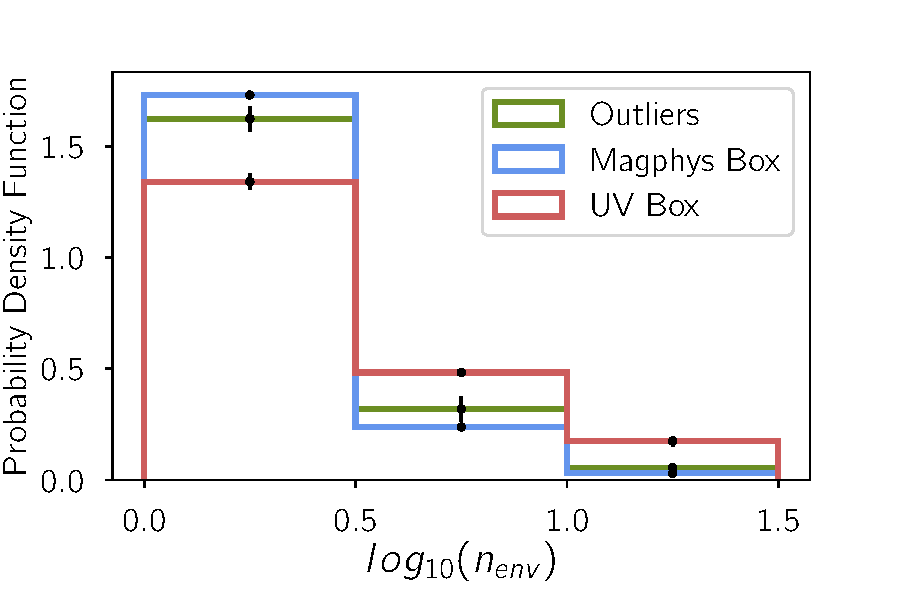
\includegraphics[width = 9 cm, height = 6.0 cm]{jk_plot.pdf}
	\caption{} 
\end{figure}



\begin{itemize}
\item{From Fig $1$, we see that MAGPHYS SSFR identifies a region in the color-color space as dust-obscured star forming galaxies and correlates better with the environments of the galaxies.}
\item{At the higher star formation end, we find that the dust-obscured star-formers as identified by MAGPHYS have environments comparable to the blue star-forming galaxies, confirming that this is indeed a physical effect we're seeing.}

\item{}
\item{}
\end{itemize}

\newpage



\begin{thebibliography}{}

\bibitem[Bruzual, G., \& Charlot, S.(2003)]{Bru03} Bruzual, G., \& Charlot, S. 2003, \mnras, 344, 1000
\bibitem[Burgarella, D. et al.(2013)]{Burg13} Burgarella, D., Buat, V., \& Gruppioni, C., et al. 2013, \aa, 554, A70
\bibitem[Calzetti, D., Kinney, A. L., \& Storchi-Bergmann, T. (1994)]{Cal94}Calzetti, D., Kinney, A. L., \& Storchi-Bergmann, T. 1994, \apj, 429, 582
\bibitem[Chabrier, G. (2003)]{Chab03} Chabrier, G. 2003, \pasp, 115, 763
\bibitem[Charlot, S. \& Fall, S. M. (2000)]{Char00}Charlot, S., \& Fall, S. M. 2000, \apj, 539, 718
\bibitem[Cooper M. C. et al.(2006)]{Coop06} Cooper M. C. et al., 2006, \mnras, 370, 198
\bibitem[da Cunha, E. et al. (2008)]{daC08} da Cunha, E., Charlot, S., \& Elbaz, D. 2008 \mnras, 388, 1595
\bibitem[Kennicutt, R. (1983)]{Ken83}Kennicutt, R. 1983, \textcolor{red}{\aj}, 120, 219
\bibitem[Kennicutt, R. C., Jr. (1998)]{Ken98} Kennicutt, R. C., Jr. 1998, \araa, 36, 189
\bibitem [Madau P. et. al. (1998)]{Mad98} Madau, P., Pozzetti, L., \& Dickinson, M. 1998, \apj, 498, 106
\bibitem[Salim, S. et al.(2007)]{Sal07} Salim, S., Rich, R. M., Charlot, S., et al., 2007, \apjs, 173, 267
\end{thebibliography}

\end{document}